%%%%%%%%%%%%%%%%%%%%%%%%%%%%%%%%%%%%%%%%%%%%%%%%%%%%%%%%%%%%%%%%%%%%%%
% LaTeX Example: Project Report
%
% Source: http://www.howtotex.com
%
% Feel free to distribute this example, but please keep the referral
% to howtotex.com
% Date: March 2011 
% 
%%%%%%%%%%%%%%%%%%%%%%%%%%%%%%%%%%%%%%%%%%%%%%%%%%%%%%%%%%%%%%%%%%%%%%
% How to use writeLaTeX: 
%
% You edit the source code here on the left, and the preview on the
% right shows you the result within a few seconds.
%
% Bookmark this page and share the URL with your co-authors. They can
% edit at the same time!
%
% You can upload figures, bibliographies, custom classes and
% styles using the files menu.
%
% If you're new to LaTeX, the wikibook is a great place to start:
% http://en.wikibooks.org/wiki/LaTeX
%
%%%%%%%%%%%%%%%%%%%%%%%%%%%%%%%%%%%%%%%%%%%%%%%%%%%%%%%%%%%%%%%%%%%%%%
% Edit the title below to update the display in My Documents
%\title{Project Report}
%
%%% Preamble
\documentclass[paper=a4, fontsize=11pt]{scrartcl}
\usepackage[T1]{fontenc}
\usepackage{xparse}
\usepackage{fourier}
\usepackage{mathtools}
\DeclarePairedDelimiter\ceil{\lceil}{\rceil}
\DeclarePairedDelimiter\floor{\lfloor}{\rfloor}
\usepackage{listings}
\usepackage[english]{babel}															% English language/hyphenation
\usepackage[protrusion=true,expansion=true]{microtype}	
\usepackage{amsmath,amsfonts,amsthm} % Math packages
\usepackage[pdftex]{graphicx}	
\usepackage{url}


%%% Custom sectioning
\usepackage{sectsty}
\allsectionsfont{\centering \normalfont\scshape}


%%% Custom headers/footers (fancyhdr package)
\usepackage{fancyhdr}
\pagestyle{fancyplain}
\fancyhead{}											% No page header
\fancyfoot[L]{}											% Empty 
\fancyfoot[C]{}											% Empty
\fancyfoot[R]{\thepage}									% Pagenumbering
\renewcommand{\headrulewidth}{0pt}			% Remove header underlines
\renewcommand{\footrulewidth}{0pt}				% Remove footer underlines
\setlength{\headheight}{13.6pt}


%%% Equation and float numbering
\numberwithin{equation}{section}		% Equationnumbering: section.eq#
\numberwithin{figure}{section}			% Figurenumbering: section.fig#
\numberwithin{table}{section}				% Tablenumbering: section.tab#


%%% Maketitle metadata
\newcommand{\horrule}[1]{\rule{\linewidth}{#1}} 	% Horizontal rule

\title{
	%\vspace{-1in} 	
	\usefont{OT1}{bch}{b}{n}
	\normalfont \normalsize \textsc{University of Illinois at Urbana-Champaign} \\ [25pt]
	\horrule{0.5pt} \\[0.4cm]
	\huge Assignment 5 - Report \\
	\horrule{2pt} \\[0.5cm]
}
\author{
	\normalfont 								\normalsize
	Department of Industrial and Enterprise Systems Engineering\\
	\normalsize Zhenye Na (zna2)\\[-3pt]		\normalsize
	\today
}
\date{}


%%% Begin document
\begin{document}
	\maketitle
	
	\section{Query Execution (25 pts)}
	
	\begin{enumerate}
		\item Consider the following relations with no indexes on them:
		\begin{itemize}
			\item Relation R has 5,000 tuples, 100 tuples per block
			\item Relation S has 2,000 tuples, unknown number of tuples per block 
		\end{itemize}
		
		The number of blocks in memory is 10. Say, S is as large as possible (within the limits that main memory can afford) for the two pass sort-merge join (slide 57). That is, if S was larger, the two pass sort-merge join would not work.
		
		Answer the following questions:
		\begin{enumerate}
			\item How many tuples per block does S have? (Do not forget to show your calculations.)\\
			\textbf{Solutions: }\\
			Number of blocks in R: $B(R) = \frac{5000}{100} = 50$\\
			Memory requirements for two pass sort-merge join is $B(R) + B(S) \leq M(M-1)$, so we can get $50 + B(S) \leq 10 \times 9$, $B(S) \geq 40 = 40$.\\
			So, we got $\frac{2000}{40} = 50$ tuples per block.
			
			\item Using your answer from A, what is the cost of joining R and S using the two pass sort-merge join algorithm (slide 57)?\\
			\textbf{Solutions: }\\
			Cost = 3B(R) + 3B(S) = 150 + 120 = 270.
			
			\item Using your answer from A, what is the cost of joining R and S using the optimized block nested-loop join algorithm?\\
			\textbf{Solutions: }\\
			Cost = $\frac{B(R)B(S)}{M-2} + \min \{B(S) ,B(R)\} = \frac{50 \times 40}{8} + 40 = 290$
			
			\item What is the cost of joining R and S using a two pass hash-based join?\\
			\textbf{Solutions: }\\
			Cost = 3B(R) + 3B(S) = 150 + 120 = 270.
			
			\item Based on questions 2, 3, and 4, explain which variant of the algorithm you would choose in terms of I/O cost. If multiple algorithms have the same I/O cost, explain other considerations that may influence your choice.\\
			\textbf{Solutions: }\\
			The I/O costs of two pass sort-merge join algorithm and two pass hash-based join algorithm are the same. However, two pass sort-merge join algorithm is more susceptible to skewed data, so I will choose two pass hash-based join algorithm.
			
		\end{enumerate}
		
	\end{enumerate}
	
	
	\section{Query Optimization (35 pts)}
	
	Consider the relations A(x,y,z), B(w,x), and C(u,v,w), with the following properties:
	\[
	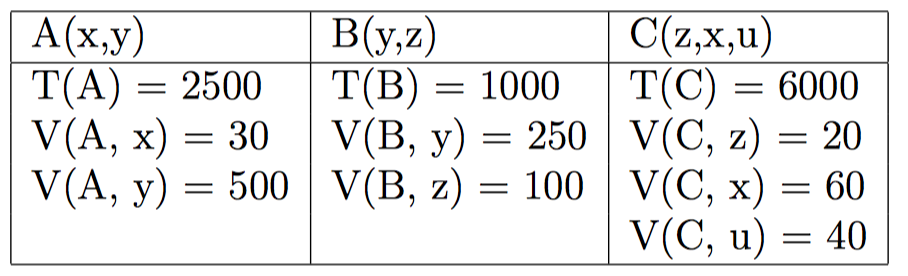
\includegraphics[scale=0.5]{1.png}
	\]
	
	where, T(R) = number of tuples in relation R and V(R, a) = number of distinct values of attribute a in relation R. Estimate the sizes (measured in number of tuples) of the result of the following expressions:
	
	\begin{enumerate}
		\item $A \times B$\\
		\textbf{Solution: }\\
		$2500 \times 6000 = 15000000$
		
		\item $A \bowtie B$\\
		\textbf{Solution: }\\
		$A \bowtie B$ is joining on column y, V(A,y)=500 > V(B,y)=250 so we loop through B.\\
		For reach tuple in B, it will join $1000 \times \frac{2500}{500} = 5000$
		So size = 5000
		
		\item SELECT u FROM C WHERE u=20\\
		\textbf{Solution: }\\
		Size will be from 0 to 5941.
		
		\item $\sigma_{x = 10 and y=30}(B \bowtie C)$\\
		\textbf{Solution: }\\
		We first compute size of $B \bowtie C$:\\
		$B \bowtie C$ will join on column z. V(B,z) = 100 > V(C,z) = 20 so we loop through C.\\
		For each tuple in C, it will join $6000 \times \frac{1000}{100} = 60000$\\
		Then we perform selection
		Size will be from 0 to (60000-250+1=59751)
		
		
	\end{enumerate}
	
	
	\section{Dynamic Programming (40 pts)}
	
	Consider the following relations, where T(R) = number of tuples in relation R and V(R, a) = number of distinct values of attribute a in relation R.
	
	\[
	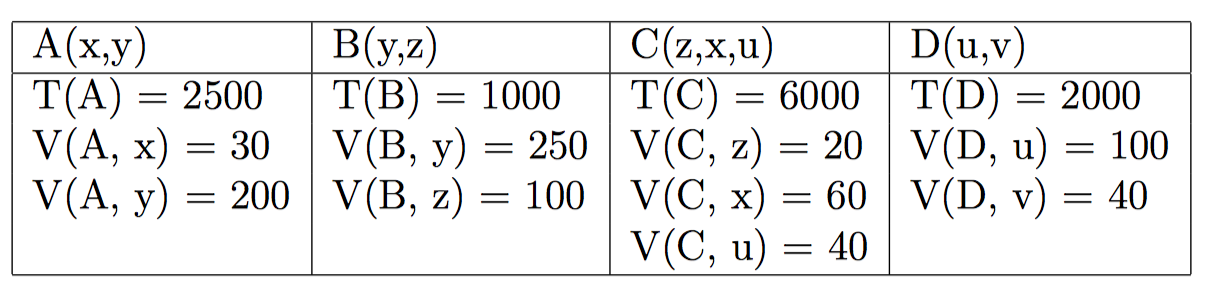
\includegraphics[scale=0.5]{2.png}
	\]
	
	We want to join all these relations as efficiently as possible. Determine the most efficient way to do the join. Clearly state any assumptions you have made. Show your work by completing the following table (each step in the dynamic programming algorithm should be one row):
	
	\[
	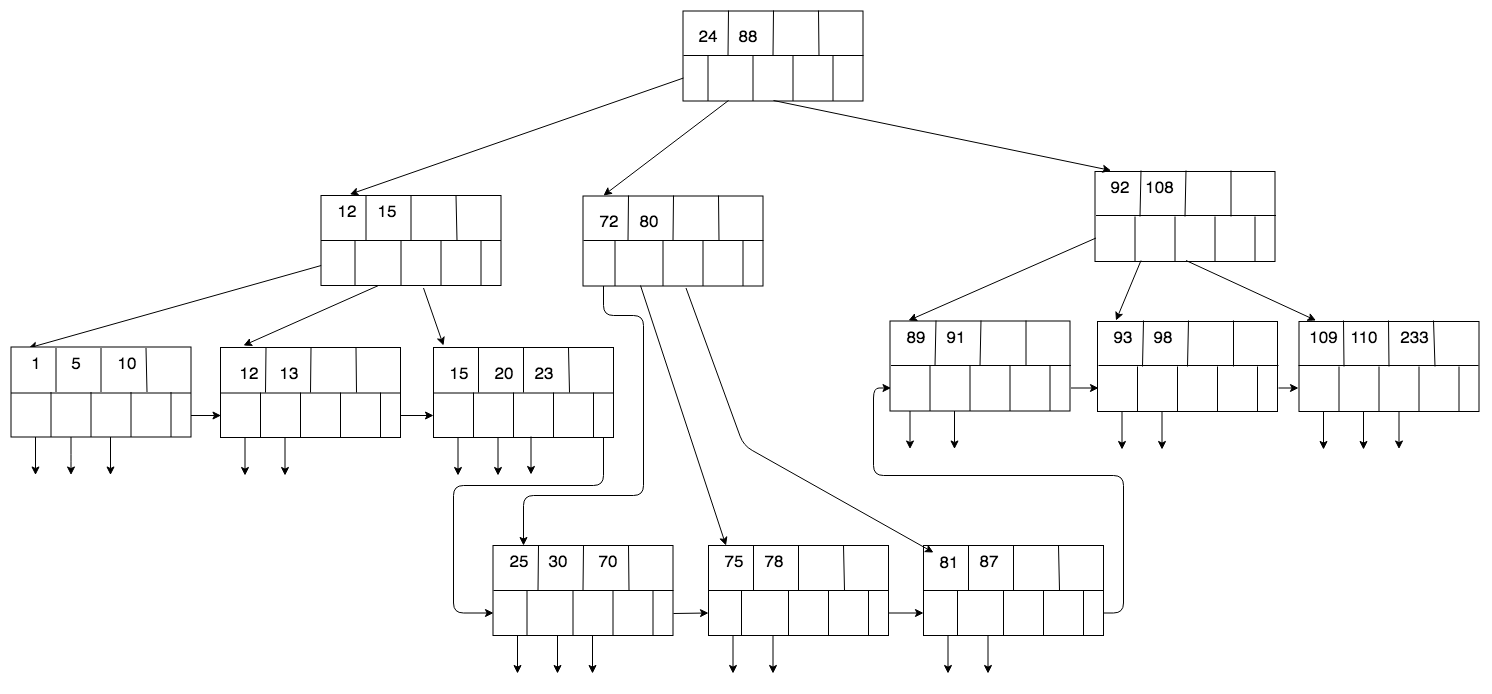
\includegraphics[scale=0.54]{3.png}
	\]
	
	\begin{table}[ht]
		\centering
		\label{Table1}
		\begin{tabular}{|c|c|c|c|}
			\hline
			\textbf{Subset} & \textbf{Size} & \textbf{Lowest Cost} & \textbf{Lowest Cost Plan} \\ \hline
			AB              & 10K           & 0                    & BA                        \\ \hline
			AC              & 250K          & 0                    & AC                        \\ \hline
			AD              & 5M            & 0                    & DA                        \\ \hline
			BC              & 60K           & 0                    & BC                        \\ \hline
			BD              & 2M            & 0                    & BD                        \\ \hline
			CD              & 120K          & 0                    & DC                        \\ \hline
			ABC             & 10K           & 10K                  & C(BA)                     \\ \hline
			ABD             & 20M           & 10K                  & D(BA)                     \\ \hline
			ACD             & 5M            & 120K                 & A(DC)                     \\ \hline
			BCD             & 1.2M          & 60K                  & D(BC)                     \\ \hline
			ABCD            & 200K          & 130K                 & (BA)(DC)                  \\ \hline
		\end{tabular}
		\caption{Dynamic Programming Table}
	\end{table}
	
	
	%%% End document
\end{document}